\documentclass{ximera}

\author{Anna Davis} \title{MTH 240 Homework 8} 

\begin{document}

\begin{abstract}

\end{abstract}
\maketitle
 \textit{Certificate due: 3/24/2021 at 11:59 p.m.}
 
\begin{problem}\label{prob:240HW8prob1}
Let $f(x)=x^3-x^2-x$.  Use the graph to find absolute extrema for each indicated interval.  If a particular type of extremum does not exist, type na in each given box.
\[
\graph[xmin=-5,xmax=5,ymin=-5,ymax=5]{f(x)=x^3-x^2-x} 
\]

\begin{enumerate}
    \item Interval: $[-1, 0]$.
    
    Absolute max is $\answer[tolerance=0.01]{0.185}$ at $x=\answer[tolerance=0.01]{-\frac{1}{3}}$.
    
    Absolute min is $\answer{-1}$ at $x=\answer{-1}$.
    
    \item Interval: $(0, 2]$.
    
    Absolute max is $\answer{2}$ at $x=\answer{2}$.
    
    Absolute min is $\answer{-1}$ at $x=\answer{1}$.
    
    \item Interval: $[0, 2)$.
    
    Absolute max is $\answer{na}$ at $x=\answer{na}$.
    
    Absolute min is $\answer{-1}$ at $x=\answer{1}$.
    
    \item Interval: $(-\infty, \infty)$.
    
    Absolute max is $\answer{na}$ at $x=\answer{na}$.
    
    Absolute min is $\answer{na}$ at $x=\answer{na}$.
\end{enumerate}
\end{problem}

\begin{problem}\label{prob:240HW8prob2}
Let $f(x)=\frac{2}{x+3}$.  Use the graph to find absolute extrema for each indicated interval.  If a particular type of extremum does not exist, type na in each given box.
\[
\graph[xmin=-5,xmax=5,ymin=-5,ymax=5]{f(x)=\frac{2}{x+3}} 
\]

\begin{enumerate}
    \item Interval: $(-3, -2]$.
    
    Absolute max is $\answer{na}$ at $x=\answer{na}$.
    
    Absolute min is $\answer{2}$ at $x=\answer{-2}$.
    
    \item Interval: $[-2, 5]$.
    
    Absolute max is $\answer{2}$ at $x=\answer{-2}$.
    
    Absolute min is $\answer{0.25}$ at $x=\answer{5}$.
    
    \item Interval: $[-6, 0]$.
    
    Absolute max is $\answer{na}$ at $x=\answer{na}$.
    
    Absolute min is $\answer{na}$ at $x=\answer{na}$.
    
    \item Interval: $[0, \infty)$.
    
    Absolute max is $\answer[tolerance=0.01]{\frac{2}{3}}$ at $x=\answer{0}$.
    
    Absolute min is $\answer{na}$ at $x=\answer{na}$.
\end{enumerate}
\end{problem}

\begin{problem}\label{prob:mth240HW8prob3}
A rectangular trough is to be constructed from a 200 ft by 12 ft sheet of metal by folding up the sides, as shown.  Use calculus to find the largest possible volume of flowing water that the trough can contain.

\begin{image}
   
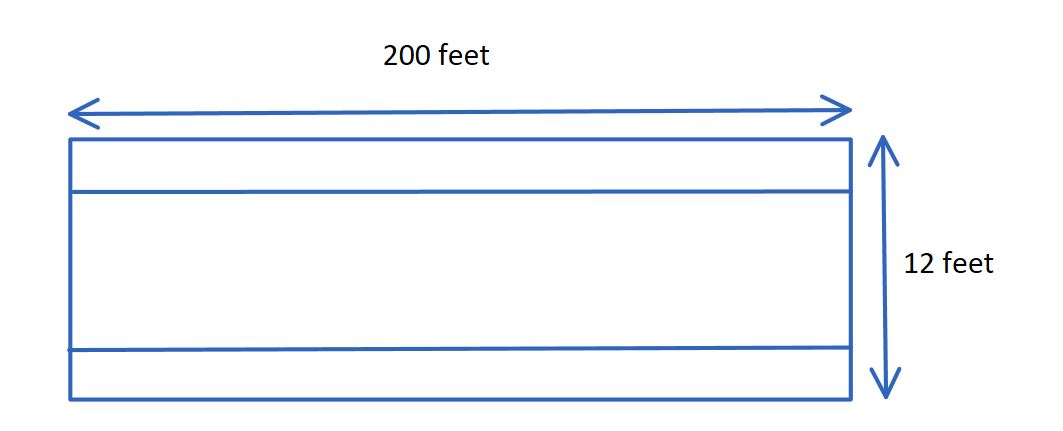
\includegraphics[height=1in]{test2image2new.jpg}~
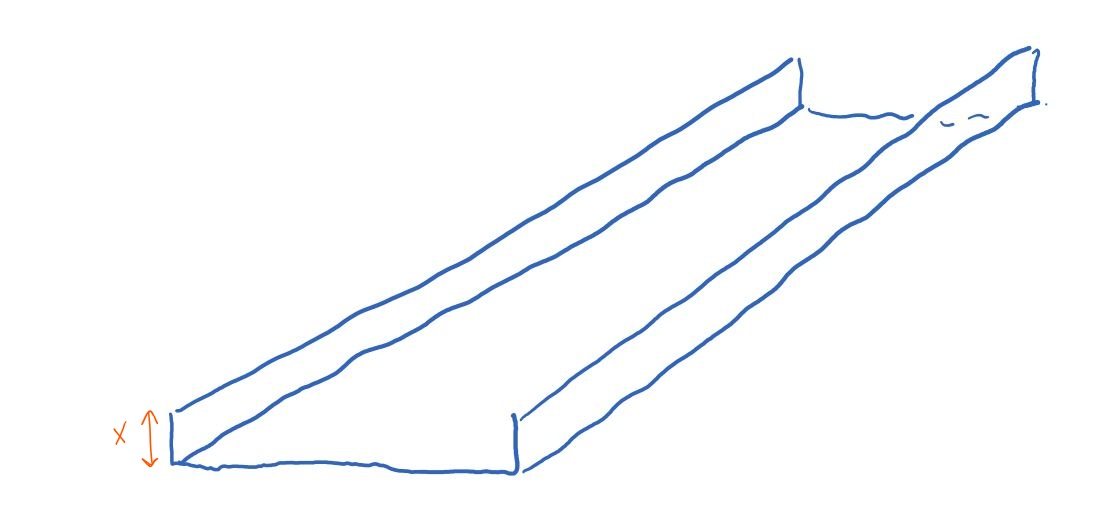
\includegraphics[height=1in]{Inkedtest2image3.jpg}~

\end{image}
Volume of the trough:
$$V(x)=\answer{200x(12-2x)}$$
Find the derivative:
$$V'(x)=\answer{-800x+2400}$$
Value of $x$ that gives the largest volume:
$$x=\answer{3}$$
Largest possible volume:
$$V=\answer{3600}\mbox{ cubic feet}$$

\end{problem}


\end{document} 